\documentclass[11pt]{beamer}
\usepackage[utf8]{inputenc}
\usepackage[T1]{fontenc}
\usetheme{default}
\usepackage{lipsum}
\usepackage{float}
\usepackage{listings}
\begin{document}
	%\author{}
	%\title{}
	%\subtitle{}
	%\logo{}
	%\institute{}
	%\date{}
	%\subject{}
	%\setbeamercovered{transparent}
	%\setbeamertemplate{navigation symbols}{}
	\frame[plain]{\maketitle}

    \begin{frame}
      \frametitle{Objetivos do Trabalho}

      O objetivo principal do trabalho foram:

      \begin{itemize}
        \item Estudar a estrutura e o funcionamento de Redes Neurais
          Convolucionais 2D
        \item Entender como a informação é transformada dentro da
            rede neural ao avançar nas camadas mais profundas
        \item Extrapolar esse conhecimento para redes mais
              clássicas como a \textbf{MLP} estudada durante a
              disciplina.
      \end{itemize}
    \end{frame}

    \begin{frame}
      \frametitle{Apresentação do Bruno}
    \end{frame}

    \begin{frame}
      \frametitle{Apresentação do Bruno Canale}
    \end{frame}

	\begin{frame}
      \frametitle{Python - Keras Framework para Machine Learning}

      * Python - Linguagem de programação gratuita \newline
      * Contém uma quantidade muito grande de Frameworks voltados para
      \textit{Machine Learning}
      

      \begin{figure}
        \centering
        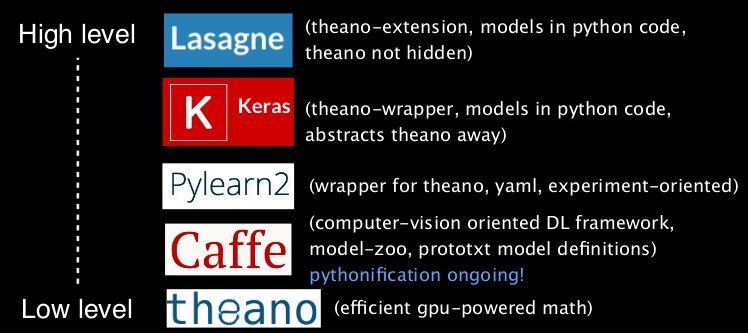
\includegraphics[scale=0.3]{road_map}
      \end{figure}

      Keras foi inicialmente desenvolvido como parte de um projeto de
      pesquisa chamado de ONEIROS (Open-ended Neuro-Electronic
      Intelligent Robot Operating System)

    \end{frame}

    \begin{frame}
      \frametitle{Keras - Exemplo de implementação MLP}

      
      modelo = Sequential() \\
      modelo.add(Dense(num-neuronios, init='uniform'))\\
      modelo.add(Activation('tanh')) \newline

      modelo.add(Dense(1, init='uniform')) \\
      modelo.add(Activation('linear')) \newline

      modelo.compile(learning-rate=0.1, optimizer='sgd]') \newline

      modelo.fit(features-treino, target-treino) \newline

      modelo.predict(features-teste)
     
    \end{frame} 
    
    \begin{frame}
      \frametitle{Base de dados utilizada - MNIST}

     \begin{columns}
       \begin{column}{0.48\textwidth}
         A base de dados MNIST é composta por 60.000 exemplos de
         imagens de digitos em letra cursivas. O dataset é ideal para
         testes de algoritmos em reconhecimentos de padrões por
         necessitar pouco pré-processamento.\\
         Mais informações no link: http://yann.lecun.com/exdb/mnist/
       \end{column}
       \begin{column}{0.48\textwidth}
         \begin{figure}
           \centering
           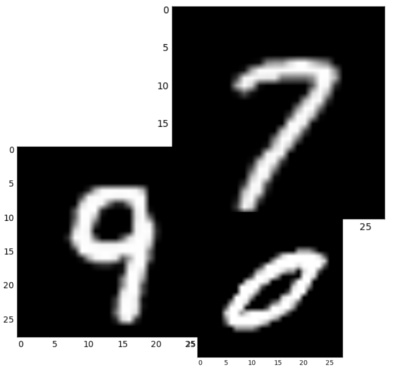
\includegraphics[scale=0.35]{minst}
           \end{figure}
       \end{column}
     \end{columns}
     
      \lstinputlisting[language=Python, firstline=0, lastline=10,
      basicstyle=\ttfamily\scriptsize]{base_import.py}
    \end{frame}

    \begin{frame}
      \frametitle{Processamento necessário no atributo target}

      Um processamento padrão é transformar o conjunto de
      \textbf{atributos targets} em um conjunto de variáveis
      categóricas. O que seriam variáveis categoricas?

      Exemplo: Se a lista de targets é composta por: [1.2, 2, 3, 4.2,
      4i] e as classes disponiveis são \textbf{real, inteiro,
        imaginario}, então uma matriz de transformação seria:
      
      \begin{table}[h]
        \caption{Conversão para variáveis categoricas}
        \begin{tabular}{l|c|c|c|}
          
          target & real & inteiro & imaginario \\
          1.2    & 1    & 0       & 0 \\
          2      & 0    & 1       & 0 \\
          3      & 0    & 1       & 0 \\
          4.2    & 1    & 0       & 0 \\
          4i     & 0    & 0       & 1
                                    
        \end{tabular}
      \end{table}
    \end{frame}

    \begin{frame}
      \frametitle{Implementação da Rede Convolucional 2D}
      \lstinputlisting[language=Python, firstline=0, lastline=25,
      basicstyle=\ttfamily\scriptsize]{cnn1.py}
    \end{frame}

    \begin{frame}
      \frametitle{Modelo do Experimento realizado para análise da
        Rede}
      \begin{itemize}
        \item Após implementação a arquitetura foi testada para
          verificar performance no conjunto de testes.
        \item Queriamos observar a transformação da imagem de Input
            após cada camada da ConvNet
        \item A fim de analisar com mais detalhes, foram adicionadas
          mais camadas convolucionais no modelo apresentado anteriormente.
        \end{itemize}
      \end{frame}
      
    
    \begin{frame}
      \frametitle{Apresentacao do Fábio - Sugestão: Introdução a exploração dos resultados}
    \end{frame}

    \begin{frame}
      \frametitle{Apresentacao do Fábio - Sugestao: Apresentacao das
        imagens dos filtros e saidas das convolucoes}
    \end{frame}

    \begin{frame}
      \frametitle{Apresentacao do Fábio - Sugestão: Discussao sobre
        como essas observacoes ligam na MLP clássica e/ou problemas de
        Machine Learning}
    \end{frame}
    
\end{document}